% =============================================================================
% CHƯƠNG 2 — NGUỒN DỮ LIỆU, MÔ HÌNH QUAN HỆ VÀ KIẾN TRÚC GIẢI PHÁP KỸ THUẬT DỮ LIỆU
% Nội dung đối chiếu với repo marketpulse-360 @ dbe614b.
% =============================================================================

\section{Nguồn dữ liệu}
\label{sec:c2-nguon-du-lieu}

Dữ liệu marketing thật luôn gắn với thông tin cá nhân và bí mật kinh doanh, nên nhóm không dùng dữ liệu của doanh nghiệp có thật. Thay vào đó, gói \texttt{marketpulse\_mock} sinh ra một ``thế giới bán lẻ'' mô phỏng có tính \emph{tất định}: cùng một \texttt{seed} và cùng một cấu hình luôn cho ra cùng một bộ file, đến từng byte. Mỗi lần sinh dữ liệu đi kèm một \texttt{manifest.json} ghi lại cấu hình, mã băm SHA-256 của từng file, số dòng, mốc thời gian và số lượng bất thường đã tiêm vào. Nhờ vậy, mọi con số trong báo cáo đều có thể tái lập và đối chiếu lại với ``sự thật gốc'' (\emph{ground truth}) của bộ sinh.

Định danh khách hàng, chiến dịch, phiên, click, đơn hàng và email được giữ nhất quán giữa các nguồn, nên dữ liệu vừa đủ ``bẩn'' để kiểm tra đường ống, vừa đủ chặt chẽ để đối soát. Bảng~\ref{tab:sources} tóm tắt các nguồn dữ liệu.

\begin{table}[!htbp]
\centering
\caption{Đặc tả các nguồn dữ liệu, định dạng, khóa liên kết và đặc trưng nổi bật}
\label{tab:sources}
\small
\renewcommand{\arraystretch}{1.2}
\begin{tabularx}{\textwidth}{>{\raggedright\arraybackslash}p{2.5cm} >{\raggedright\arraybackslash}p{2.2cm} >{\raggedright\arraybackslash}p{4.8cm} >{\raggedright\arraybackslash}X}
\toprule
\textbf{Nguồn} & \textbf{Định dạng / kênh} & \textbf{Khóa liên kết} & \textbf{Đặc trưng} \\
\midrule
\texttt{web\_events} & JSONL, Kafka thời gian thực & \texttt{event\_id}, \texttt{session\_id}, \texttt{customer\_id} hoặc \texttt{anonymous\_id}, \texttt{click\_id}, \texttt{campaign\_id} & 5 loại sự kiện phễu từ web và ứng dụng; có trùng lặp, đến trễ, phiên bot \\
\texttt{orders} & JSONL, Kafka thời gian thực & \texttt{order\_id}, \texttt{customer\_id} & \texttt{order\_created}, \texttt{order\_refunded}; số tiền là số nguyên VND \\
\texttt{email\_events} & JSONL, Kafka thời gian thực & \texttt{message\_id}, \texttt{customer\_id}, mã chiến dịch vòng đời & Gửi, nhận, mở, click, hủy đăng ký \\
\texttt{google\_ads} & CSV theo ngày & mã chiến dịch của nền tảng & Chi phí tính bằng \texttt{cost\_micros} \\
\texttt{meta\_ads} & JSONL theo ngày & mã chiến dịch của nền tảng & Chi phí là chuỗi thập phân, có cặp \texttt{date\_start}/\texttt{date\_stop} \\
\texttt{tiktok\_ads} & CSV theo ngày & mã chiến dịch của nền tảng & Ngày ghi ở trường \texttt{stat\_time\_day} \\
\texttt{shopee\_ads} & CSV theo ngày & mã quảng cáo & Ngày dạng \texttt{DD/MM/YYYY}, chi phí ở trường \texttt{expense} \\
\texttt{crm} & CSV, ảnh chụp hằng ngày & \texttt{customer\_id} & Hạng thành viên, giá trị vòng đời, cờ đồng thuận \\
\texttt{master/*} & CSV & \texttt{campaign\_id}, \texttt{ad\_id}, \texttt{customer\_id}, \texttt{product\_id} & Danh mục chiến dịch, quảng cáo, khách hàng, sản phẩm \\
\bottomrule
\end{tabularx}
\end{table}

\subsection{Luồng sự kiện thời gian thực}
\label{sec:c2-luong-su-kien}

Ba luồng sự kiện được phát lại vào Kafka theo đúng thứ tự thời gian bởi công cụ \texttt{replay}. Luồng \texttt{web\_events} mô tả hành trình mua sắm trên web và ứng dụng qua năm sự kiện \texttt{page\_view}, \texttt{view\_item}, \texttt{add\_to\_cart}, \texttt{begin\_checkout} và \texttt{purchase}; các phiên đến từ quảng cáo trả phí mang theo \texttt{click\_id} và \texttt{campaign\_id}. Luồng \texttt{orders} ghi nhận giao dịch tài chính qua \texttt{order\_created} và \texttt{order\_refunded}. Luồng \texttt{email\_events} theo dõi vòng đời một email qua \texttt{email\_sent}, \texttt{email\_delivered}, \texttt{email\_opened}, \texttt{email\_clicked} và \texttt{email\_unsubscribed}.

Công cụ phát lại có hai đặc điểm quan trọng cho tính đúng. Thứ nhất, producer bật \texttt{enable.idempotence} và \texttt{acks=all}, nên khi một lần gửi gặp lỗi mạng và producer tự gửi lại trong cùng phiên làm việc, Kafka không ghi thêm bản sao. Chế độ này không loại được bản ghi trùng có sẵn trong dữ liệu nguồn, vốn được tiêm có chủ đích (Mục~\ref{sec:c2-veracity}); việc khử trùng lặp do Flink và tầng Silver đảm nhận. Thứ hai, con trỏ phát lại được gắn với mã băm của manifest: nếu thế giới dữ liệu thay đổi, con trỏ cũ sẽ bị từ chối thay vì âm thầm tiếp tục trên một tập dữ liệu khác.

\subsection{Dữ liệu lô theo lịch}
\label{sec:c2-du-lieu-lo}

Nhóm dữ liệu lô mô phỏng đúng cách các nền tảng quảng cáo xuất báo cáo trong thực tế: mỗi nền tảng một định dạng, một cách ghi ngày và một đơn vị tiền riêng (Bảng~\ref{tab:sources}). Bên cạnh đó là ảnh chụp CRM hằng ngày và bốn bảng danh mục \texttt{master/campaigns}, \texttt{master/ads}, \texttt{master/customers}, \texttt{master/products}. Tầng Silver chịu trách nhiệm chuẩn hóa toàn bộ các khác biệt này về một mô hình chung, quy chi phí về số nguyên VND bằng làm tròn \emph{half-up}, và từ chối cả lô nếu có báo cáo chi phí không ánh xạ được về chiến dịch nào.

\subsection{Các quy mô dữ liệu}
\label{sec:c2-profiles}

Bộ sinh hỗ trợ nhiều cấu hình quy mô, phục vụ những mục đích khác nhau:

\begin{itemize}
    \item \textbf{fixture}: \num{615} dòng trong 22 file nén, được lưu ngay trong kho mã để kiểm thử tự động và tái lập nhanh.
    \item \textbf{demo}: \num{1200225} dòng trong 130 file (khoảng 90\,MB) với \texttt{seed} 360, dùng để kiểm tra đường ống ở quy mô vừa.
    \item \textbf{story-demo}: kịch bản \texttt{vietnam-retail} kéo dài 638 ngày, từ 01/01/2025 đến 30/09/2026, gồm \num{2576737} dòng trong \num{6342} file. Kịch bản mô phỏng 13 tỉnh/thành phố, bốn kênh quảng cáo (kể cả Shopee Ads), nhịp truy cập theo giờ Việt Nam (GMT+7), các đợt cao điểm như 11/11, Black Friday và Tết, cùng lưu lượng tự nhiên, trực tiếp và từ email. Đây là bộ dữ liệu dùng cho phần minh chứng ứng dụng ở Chương~\ref{chap:ung-dung}.
\end{itemize}

\section{Đặc trưng 4V}
\label{sec:c2-4v}

\subsection{Khối lượng (Volume)}
\label{sec:c2-volume}
Ở quy mô story-demo, hệ thống lưu trữ và xử lý hơn 2,5 triệu bản ghi nguồn, trong đó riêng lịch sử sự kiện đến 31/08/2026 đã có \num{1202050} sự kiện, và lớp hành trình khách hàng sau quản trị còn \num{1164717} sự kiện hợp lệ. Khối lượng này đủ lớn để các lựa chọn về phân vùng bảng, định dạng cột và tách biệt tính toán--lưu trữ tạo ra khác biệt rõ rệt về chi phí xử lý; phần đánh giá ở Chương~\ref{chap:danh-gia} còn mở rộng tầng phục vụ lên 20 triệu dòng.

\subsection{Tốc độ (Velocity)}
\label{sec:c2-velocity}
Sự kiện hành vi và đơn hàng đến liên tục, không theo lô. Khi phát lại lịch sử ở chế độ không giãn cách, toàn bộ \num{1202050} sự kiện được đẩy vào Kafka trong khoảng 32 giây, tức hơn \num{37000} sự kiện mỗi giây, và Flink theo kịp với độ trễ tiêu thụ (consumer lag) bằng 0. Ở chế độ trình diễn liên tục, tháng 09/2026 được phát lại với tốc độ gấp 20 lần thời gian thực để quan sát số liệu trực tiếp.

\subsection{Đa dạng (Variety)}
\label{sec:c2-variety}
Dữ liệu đến từ chín loại nguồn với hai định dạng (CSV và JSONL), hai kiểu thời gian (luồng và ảnh chụp theo ngày), ba cách ghi ngày, ba cách biểu diễn tiền tệ và nhiều loại định danh (khách hàng đã đăng nhập, khách ẩn danh, phiên, click, đơn hàng, email). Thách thức lớn nhất của sự đa dạng là \emph{hợp nhất định danh}: một khách hàng có thể bắt đầu ẩn danh trên ứng dụng, click quảng cáo trên web rồi đăng nhập khi thanh toán.

\subsection{Độ tin cậy (Veracity)}
\label{sec:c2-veracity}
Để kiểm chứng khả năng tự vệ của đường ống, bộ sinh tiêm nhiễu theo các tỷ lệ mặc định trong \texttt{DEFAULT\_ANOMALY\_RATES}: 0,5\% sự kiện trùng lặp, 1,0\% sự kiện đến trễ, 0,2\% bản ghi sai quy cách, 0,2\% phiên bot, 5,0\% khách hàng từ chối đồng thuận phân tích và 5,0\% đơn hàng bị hoàn tiền. Mỗi loại nhiễu có một cơ chế xử lý riêng ở những tầng khác nhau của đường ống, và số lượng thực tế của từng loại được ghi trong manifest để đối soát sau xử lý.

\section{Kiến trúc tổng thể}
\label{sec:c2-kien-truc}

\subsection{Vòng đời dữ liệu bốn giai đoạn}
\label{sec:c2-vong-doi}
Dữ liệu trong MarketPulse 360 đi qua bốn giai đoạn: \emph{thu thập} (Kafka và kho lưu trữ đối tượng MinIO), \emph{xử lý} (Flink cho luồng, Spark cho lô), \emph{lưu trữ} (Iceberg cho lịch sử, ClickHouse cho phục vụ phân tích, PostgreSQL cho dữ liệu vận hành) và \emph{phân phối} (FastAPI và giao diện Next.js). Điểm then chốt của kiến trúc là cả hai nhánh xử lý đều bắt nguồn từ \emph{cùng một trục sự kiện Kafka} (Hình~\ref{fig:architecture}), nên số liệu trực tiếp và số liệu lịch sử được tính từ cùng một nguồn. Hai nhánh không hoàn toàn độc lập: nhánh lô lưu vào Bronze cả topic \texttt{raw} lẫn đầu ra \texttt{clean} và DLQ của Flink, rồi dựng tầng Silver từ đầu ra của Flink. Mục~\ref{sec:c3-lakehouse-co-che} phân tích hệ quả của sự phụ thuộc này. Hai thành phần dùng chung cho cả hai nhánh là Apicurio Registry, nơi lưu hợp đồng dữ liệu của các topic, và cặp Prometheus, Grafana, thu chỉ số vận hành của Kafka, Flink, ClickHouse và API năm giây một lần để phục vụ giám sát và cảnh báo.

\begin{figure}[H]
    \centering
    \resizebox{\textwidth}{!}{% Hình 2.1 — Kiến trúc tổng thể kết hợp Streaming và Batch
\begin{tikzpicture}[b/.style={mpbox=27mm, minimum height=15mm}, h/.style={mphead=27mm, minimum height=15mm}]
  % Nhánh luồng
  \node[b] (s0) at (0,0)    {\textbf{Sự kiện}\\ web, app,\\ đơn hàng, email};
  \node[b] (k1) at (3.6,0)  {\textbf{Apache Kafka}\\ topic \texttt{raw}};
  \node[h] (fl) at (7.2,0)  {Apache Flink\\ \scriptsize\mdseries kiểm tra, khử trùng,\\ \scriptsize\mdseries gom phiên, chỉ số};
  \node[b] (k2) at (10.8,0) {\textbf{Apache Kafka}\\ topic \texttt{clean}, \texttt{gold}};
  \node[b] (lv) at (14.4,0) {\textbf{Serving workers}\\ ghi vào\\ ClickHouse live};
  % Hợp đồng dữ liệu cho các topic
  \node[mpbox=27mm] (ap) at (3.6,2.4) {\textbf{Apicurio Registry}\\ hợp đồng JSON Schema};
  % Nhánh lô
  \node[b] (b0) at (0,-3.4)    {\textbf{Quảng cáo,}\\ \textbf{CRM, danh mục}\\ (CSV/JSONL)};
  \node[b] (br) at (3.6,-3.4)  {\textbf{Bronze}\\ Spark + Iceberg\\ trên MinIO};
  \node[h] (sg) at (7.2,-3.4)  {Silver $\rightarrow$ Gold\\ \scriptsize\mdseries Spark, Iceberg, Nessie};
  \node[b] (rc) at (10.8,-3.4) {\textbf{Release ứng viên}\\ ClickHouse,\\ dbt và đối soát};
  \node[b] (pb) at (14.4,-3.4) {\textbf{Công bố}\\ \textbf{nguyên tử}\\ sổ cái PostgreSQL};
  \node[mpbox=135mm] (dg) at (9.0,-5.5) {\textbf{Dagster}: điều phối nhánh lô hằng ngày lúc 02:00, từ nạp Bronze đến công bố};
  % Ứng dụng và giám sát
  \node[mphead=24mm, minimum height=20mm] (app) at (18.2,-1.7) {Command\\ Center\\[2pt] \scriptsize\mdseries FastAPI + Next.js};
  \node[mpbox=24mm] (mon) at (18.2,2.4) {\textbf{Giám sát}\\ Prometheus + Grafana\\ \scriptsize Kafka, Flink,\\ \scriptsize ClickHouse, API};

  \begin{scope}[on background layer]
    \node[mpzone, fit=(s0)(lv)(ap)] (zs) {};
    \node[mpzone, fit=(b0)(pb)(dg)] (zb) {};
  \end{scope}
  \node[mpzonelabel, anchor=south west] at (zs.north west) {Nhánh luồng (Streaming): độ trễ thấp, số liệu tạm thời};
  \node[mpzonelabel, anchor=north west] at (zb.south west) {Nhánh lô (Batch): lịch sử đầy đủ, số liệu đã kiểm chứng};

  \draw[mparrow] (s0) -- (k1);
  \draw[mparrow] (k1) -- (fl);
  \draw[mparrow] (fl) -- (k2);
  \draw[mparrow] (k2) -- (lv);
  \draw[mparrow] (b0) -- (br);
  \draw[mparrow] (br) -- (sg);
  \draw[mparrow] (sg) -- (rc);
  \draw[mparrow] (rc) -- (pb);
  \draw[mparrow] (lv.east) -- ++(0.6,0) |- ([yshift=4mm]app.west);
  \draw[mparrow] (pb.east) -- ++(0.6,0) |- ([yshift=-4mm]app.west);
  % Hợp đồng, điều phối và giám sát
  \draw[mpdash] (ap) -- node[right, mpnote] {kiểm tra hợp đồng} (k1);
  \foreach \n in {br, sg, rc, pb} \draw[mpdash] (\n.south |- dg.north) -- (\n.south);
  \draw[mpdash] (mon.west -| zs.east) -- (mon.west);
  % Nhánh lô lưu vào Bronze cả topic raw lẫn đầu ra clean và DLQ của Flink
  \draw[mpdash] (k1.south) -- node[left, mpnote, pos=0.5] {Spark đọc \texttt{read\_committed}} (br.north);
  \draw[mpdash] (k2.south) -- ++(0,-0.55) -| node[pos=0.25, below, mpnote, align=center] {\texttt{clean.customer-events}\\ \texttt{dlq.flink-validation}} ([xshift=4mm]br.north);
\end{tikzpicture}
}
    \caption{Kiến trúc tổng thể kết hợp Streaming và Batch}
    \label{fig:architecture}
\end{figure}

\subsection{Nhánh luồng (Streaming)}
\label{sec:c2-streaming}
Flink đọc các topic \texttt{raw}, kiểm tra hợp đồng dữ liệu, khử trùng lặp, phân loại sự kiện trễ, gom phiên và cập nhật chỉ số theo chiến dịch, rồi ghi kết quả ra các topic \texttt{clean} và \texttt{gold} với bảo đảm \emph{exactly-once}. Hai tiến trình nền của ứng dụng đọc các topic này và nạp vào cơ sở dữ liệu \texttt{marketpulse\_live} trên ClickHouse. Số liệu ở nhánh này có độ trễ vài giây nhưng mang tính tạm thời: chưa có chi phí quảng cáo và chưa được đối soát. Mức quản trị cũng khác nhau giữa hai nơi đọc dữ liệu: chỉ số chiến dịch do Flink tính chưa loại sự kiện thiếu đồng thuận phân tích và phiên bot, còn màn hình Live View áp dụng đúng quy tắc của tầng Silver (khử trùng, lọc đồng thuận, loại phiên bot) ngay khi truy vấn.

\subsection{Nhánh lô (Batch)}
\label{sec:c2-batch}
Theo lịch hằng ngày, Dagster điều phối Spark lưu trữ bất biến các bản ghi Kafka và các file báo cáo vào tầng Bronze, xây dựng tầng Silver và Gold trên Iceberg, xuất snapshot sang một cơ sở dữ liệu ClickHouse ứng viên, chạy \texttt{dbt build} cùng bộ đối soát, rồi mới công bố. Nhánh này chậm hơn nhưng đầy đủ hơn: có chi phí quảng cáo từ cả bốn nền tảng, áp dụng toàn bộ quy tắc quản trị và được đối soát trước khi công bố. Về sự kiện đến trễ, nhánh lô kế thừa cách phân loại của Flink: sự kiện trễ trong ngưỡng sửa 10 phút được tính, còn sự kiện trễ hơn bị loại ở cả hai nhánh. Giao diện luôn ghi rõ con số nào thuộc nhánh nào.

\section{Mô hình dữ liệu Medallion}
\label{sec:c2-medallion}

Hồ dữ liệu được tổ chức theo kiến trúc Medallion gồm 15 bảng Iceberg (Hình~\ref{fig:medallion}). Mỗi tầng có một trách nhiệm rõ ràng: Bronze giữ nguyên bản gốc để có thể phát lại và tính lại; Silver làm sạch, chuẩn hóa và quản trị; Gold tổng hợp sẵn cho các câu hỏi nghiệp vụ. Toàn bộ lược đồ được khai báo một lần trong \texttt{contracts.py} và dùng chung cho cả mã xây dựng bảng lẫn mã kiểm chứng.

\begin{figure}[!htbp]
    \centering
    \resizebox{\textwidth}{!}{\input{chapters/Figs/fig-medallion}}
    \caption{Luồng biến đổi dữ liệu Medallion Bronze $\rightarrow$ Silver $\rightarrow$ Gold}
    \label{fig:medallion}
\end{figure}

Trong các lược đồ quan hệ của báo cáo, khóa được ký hiệu \texttt{PK} (khóa chính), \texttt{FK} (khóa ngoại; chỉ số \texttt{FK1}, \texttt{FK2}\ldots{} phân biệt các khóa ngoại trong cùng bảng) và \texttt{UK} (khóa duy nhất/khóa tự nhiên). Kiểu kèm chữ \texttt{NULL} là cột cho phép rỗng; các cột còn lại đều \texttt{NOT NULL}. Đường nét liền biểu diễn khóa ngoại, nét đứt biểu diễn tham chiếu không có ràng buộc (qua trường JSON hoặc tra cứu ở tầng ứng dụng), nét chấm có mũi tên biểu diễn quan hệ dẫn xuất. Với Iceberg và ClickHouse, khóa là \emph{logic}: động cơ lưu trữ không cưỡng chế, nhưng đường ống kiểm tra chúng ở mỗi lần xây dựng.

\subsection{Tầng Bronze: dữ liệu gốc bất biến}
\label{sec:c2-bronze}

Tầng Bronze gồm ba bảng (Hình~\ref{fig:schema-bronze}). Bảng \texttt{bronze.kafka\_records} lưu nguyên văn từng bản ghi Kafka (khóa, header và payload dạng base64 kèm mã băm) cùng tọa độ \texttt{(source\_topic, source\_partition, source\_offset)}. Khóa \texttt{ingest\_id} được tính bằng SHA-256 của chính bộ tọa độ này, nên việc nạp lại cùng một khoảng offset không bao giờ tạo bản ghi trùng. Với dữ liệu file, \texttt{bronze.source\_files} ghi mỗi file nguồn một dòng, khóa là mã băm nội dung \texttt{file\_sha256}; file gốc được lưu vào MinIO theo địa chỉ nội dung. Bảng \texttt{bronze.source\_file\_rows} lưu từng dòng của file dưới dạng JSON, liên kết về file cha qua \texttt{file\_sha256} theo quan hệ một--nhiều. Các bảng được phân vùng theo ngày Kafka hoặc theo tập dữ liệu và ngày nguồn để truy vấn lịch sử chỉ quét đúng phần cần thiết.

\begin{figure}[H]
    \centering
    \includegraphics[width=0.92\textwidth]{chapters/Pics/schema-bronze.png}
    \caption{Lược đồ quan hệ tầng Bronze}
    \label{fig:schema-bronze}
\end{figure}

\subsection{Tầng Silver: dữ liệu chuẩn hóa}
\label{sec:c2-silver}

Tầng Silver gồm sáu bảng, trình bày trong hai hình: Hình~\ref{fig:schema-silver} gồm bảng sự kiện và ba bảng danh mục, Hình~\ref{fig:schema-silver-2} gồm bảng chi phí quảng cáo và bảng thống kê chất lượng. Trung tâm là \texttt{silver.customer\_events} với 26 cột: mỗi sự kiện hợp lệ xuất hiện đúng một lần theo \texttt{event\_id}, mang \texttt{profile\_key} đã hợp nhất (\texttt{customer:}, \texttt{anonymous:} hoặc \texttt{session:}), cờ bot, trạng thái đến trễ, và bộ ba lineage \texttt{(lineage\_topic, lineage\_partition, lineage\_offset)} trỏ ngược về đúng bản ghi gốc trong Bronze. Ba bảng danh mục \texttt{silver.campaigns}, \texttt{silver.customers}, \texttt{silver.products} cùng bảng chi phí \texttt{silver.ad\_spend\_daily} đều giữ lineage \texttt{(source\_file, source\_row\_number)} về dòng nguồn. Bảng \texttt{silver.quality\_summary} đếm số bản ghi theo ngày, topic và mã lý do (chấp nhận, trùng lặp, sai quy cách, từ chối đồng thuận, bot\ldots), là đầu vào cho màn hình sức khỏe dữ liệu.

Quan hệ giữa các bảng được kiểm tra ngay khi xây dựng: chi phí không ánh xạ được về chiến dịch làm thất bại cả lô, khách hàng trong CRM phải tồn tại trong danh mục khách hàng, và mã \texttt{platform\_campaign\_id} phải duy nhất.

\begin{figure}[!htbp]
    \centering
    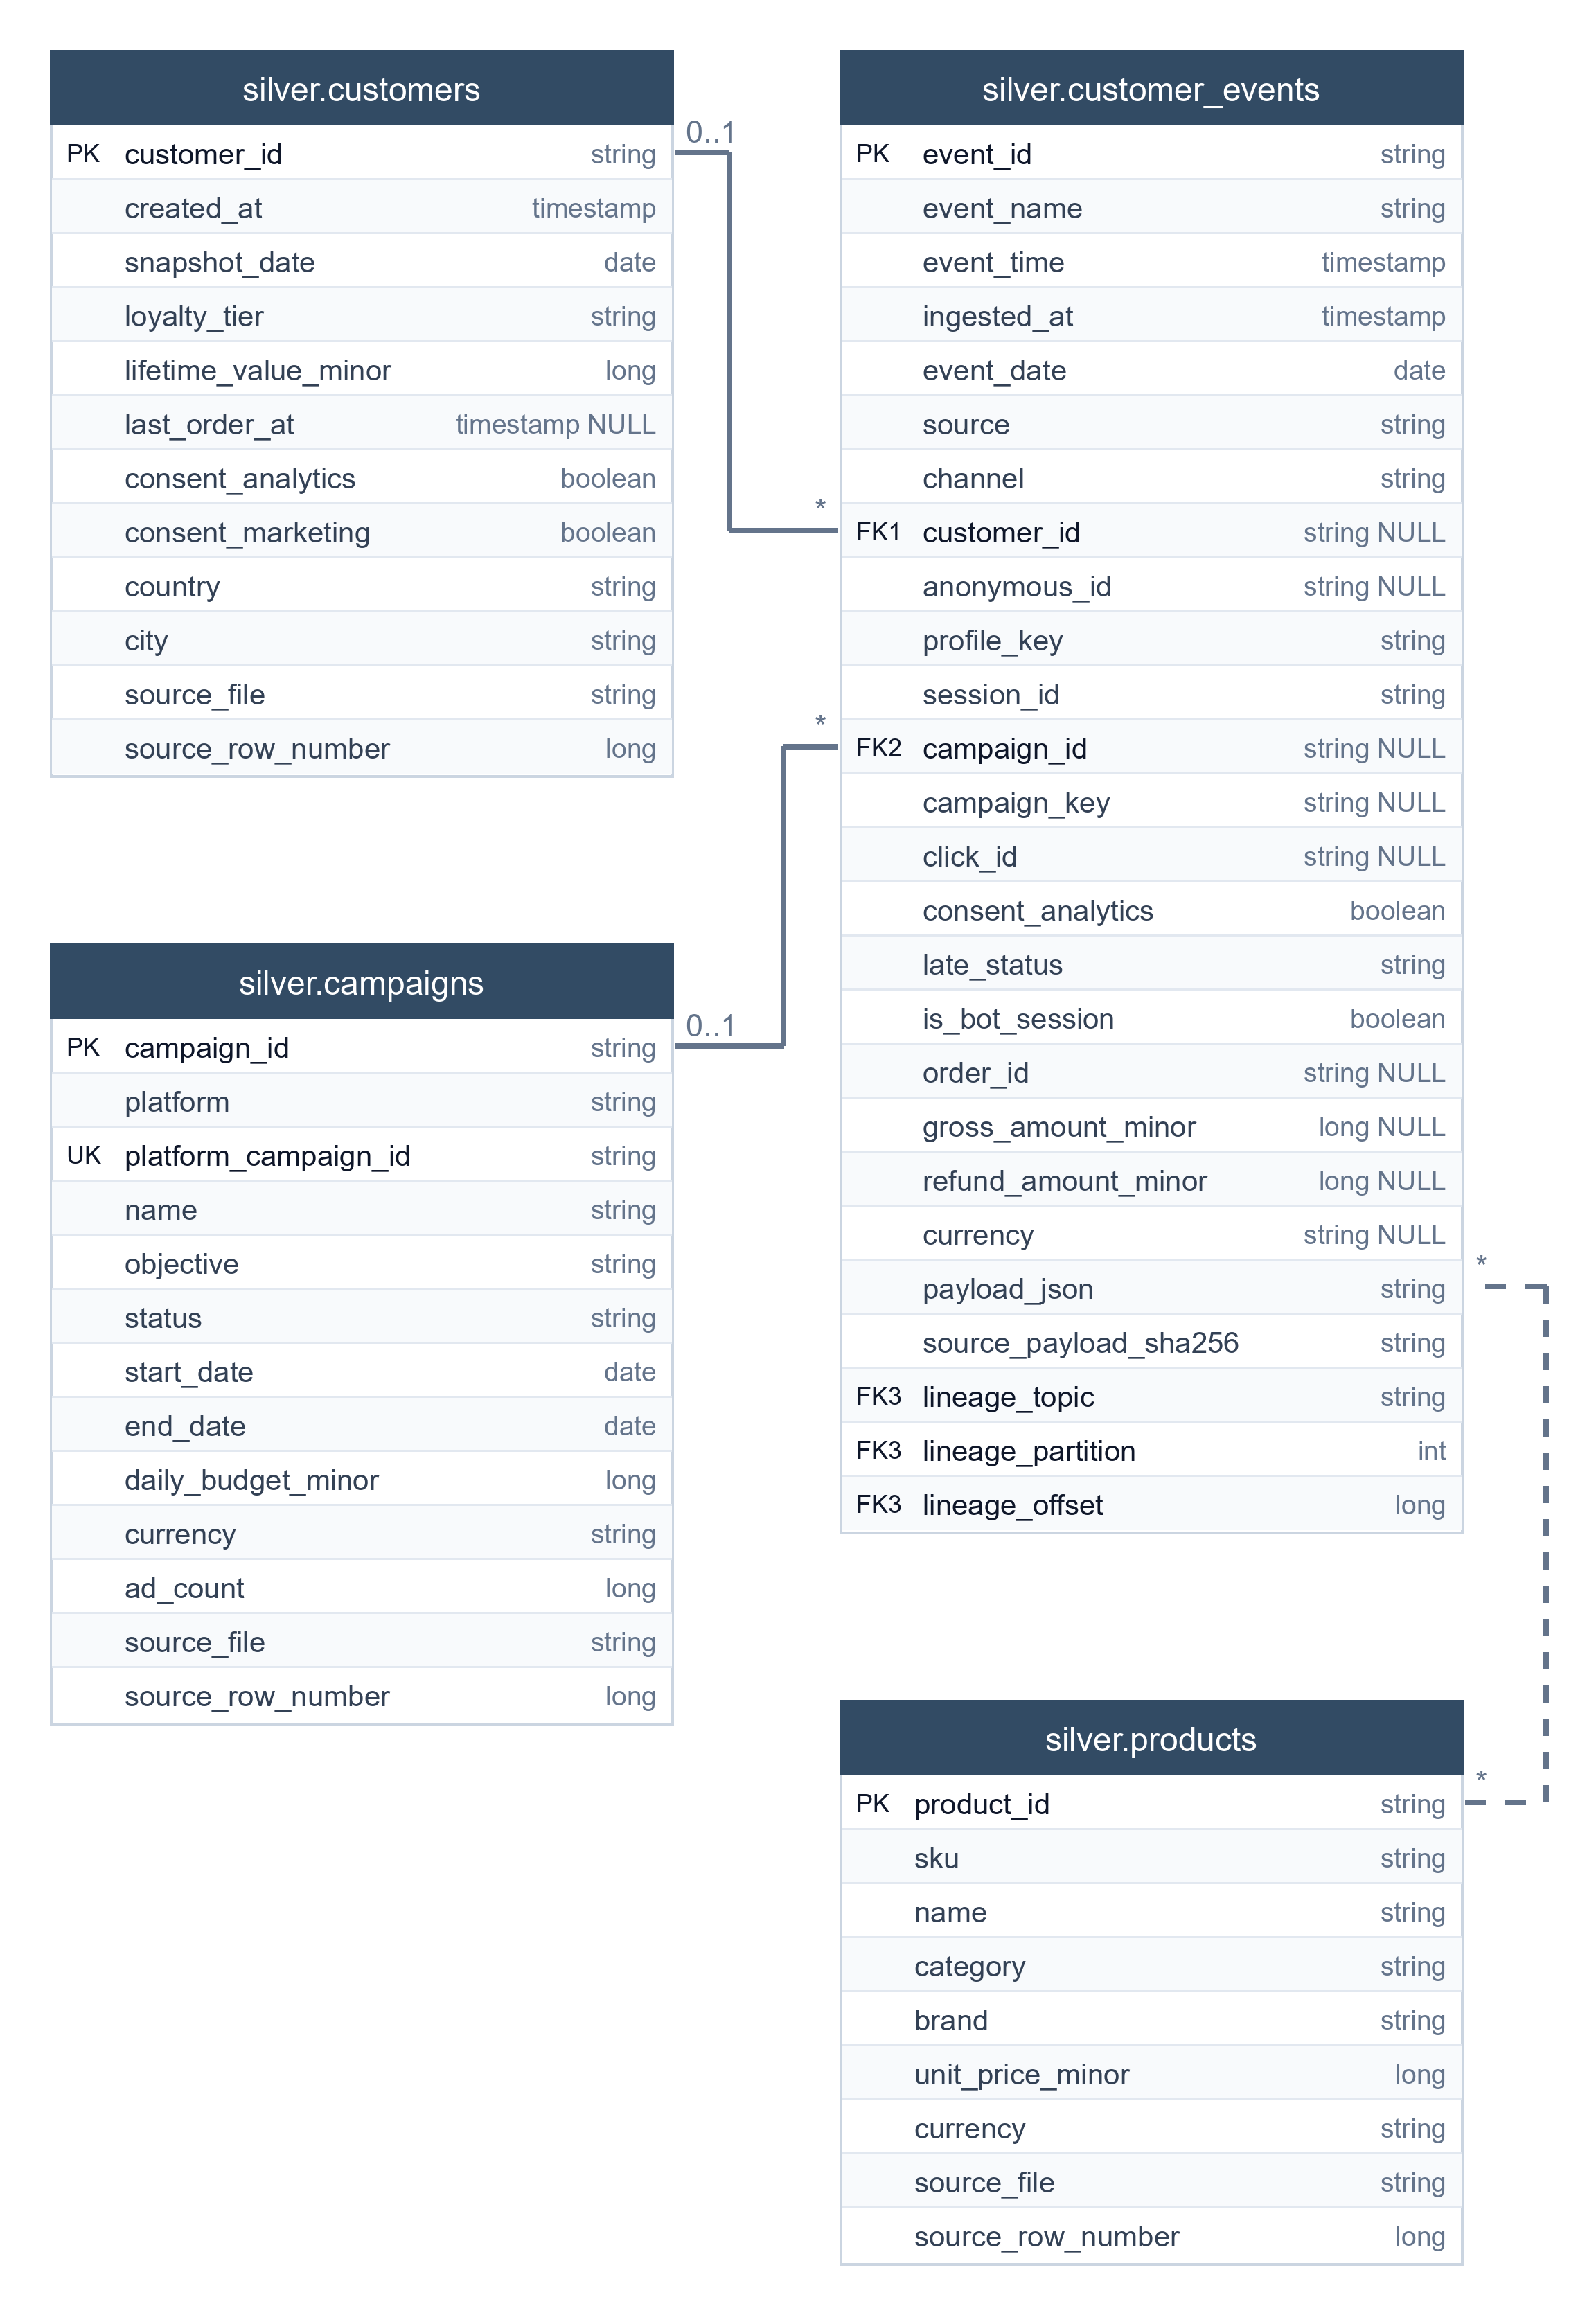
\includegraphics[width=\textwidth, height=0.86\textheight, keepaspectratio]{chapters/Pics/schema-silver-1.png}
    \caption{Lược đồ quan hệ tầng Silver (phần 1): sự kiện khách hàng và các bảng danh mục}
    \label{fig:schema-silver}
\end{figure}

\begin{figure}[!htbp]
    \centering
    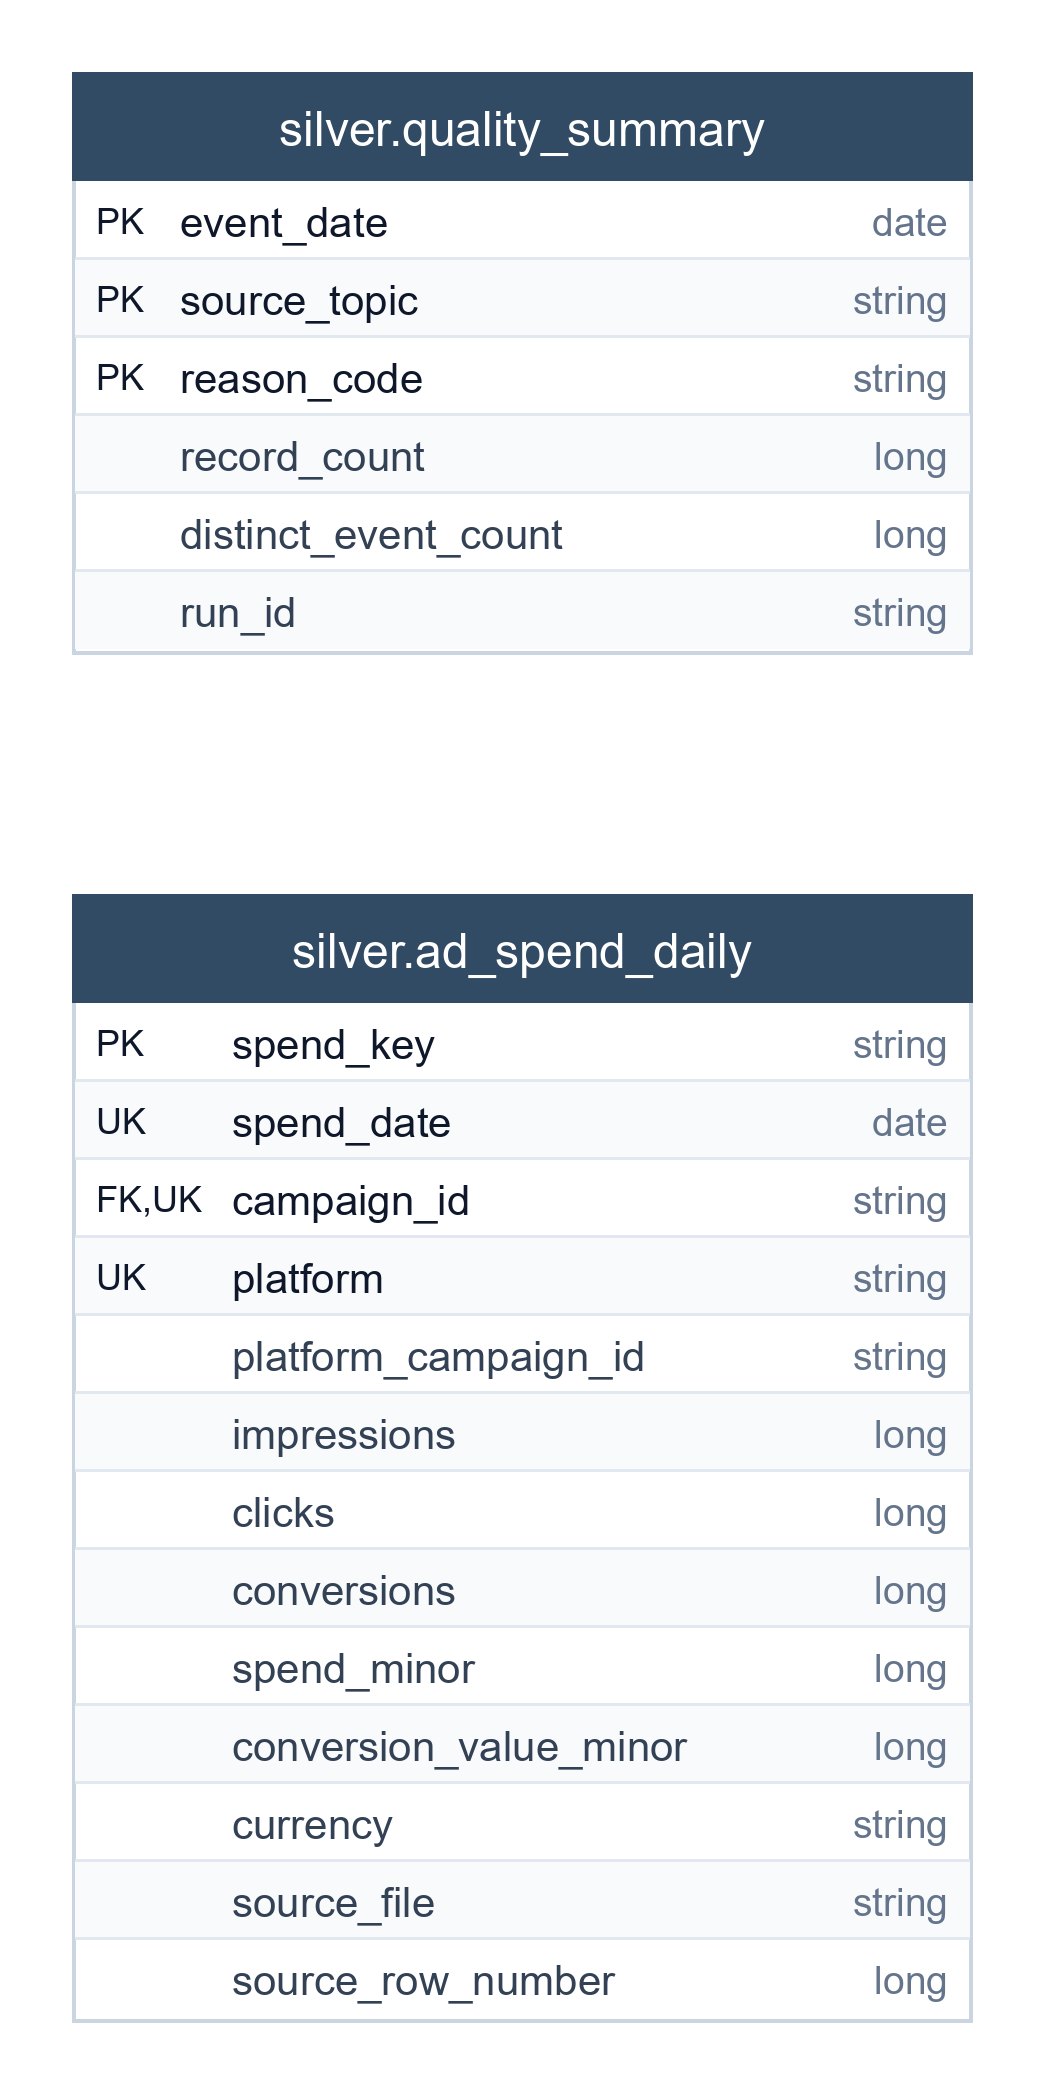
\includegraphics[width=0.42\textwidth]{chapters/Pics/schema-silver-2.png}
    \caption[Lược đồ quan hệ tầng Silver (phần 2): chi phí quảng cáo và thống kê chất lượng]{Lược đồ quan hệ tầng Silver (phần 2): chi phí quảng cáo và thống kê chất lượng. Khóa ngoại \texttt{campaign\_id} của \texttt{silver.ad\_spend\_daily} trỏ tới \texttt{silver.campaigns} ở Hình~\ref{fig:schema-silver}}
    \label{fig:schema-silver-2}
\end{figure}

\section{Lựa chọn lưu trữ và phương án thay thế}
\label{sec:c2-luu-tru-thay-the}

\subsection{Phân tách lưu trữ theo tải truy cập}
\label{sec:c2-phan-tach-luu-tru}

MarketPulse 360 không dùng một cơ sở dữ liệu cho mọi việc. Mỗi kiểu tải truy cập được giao cho hệ thống phù hợp nhất (Bảng~\ref{tab:components}): kho đối tượng giá rẻ cho dữ liệu gốc, định dạng bảng có giao dịch cho lịch sử, CSDL cột cho truy vấn phân tích độ trễ thấp và CSDL quan hệ cho dữ liệu vận hành cần ràng buộc chặt. Nhờ tách biệt, việc tính lại toàn bộ lịch sử trên Spark không ảnh hưởng đến người dùng đang đọc ClickHouse, và dữ liệu nghiệp vụ của ứng dụng (tài khoản, cấu hình, phân đoạn) không lẫn vào kho phân tích.

\begin{table}[!htbp]
\centering
\caption{Vai trò của các thành phần xử lý, lưu trữ và giám sát}
\label{tab:components}
\small
\renewcommand{\arraystretch}{1.2}
\begin{tabularx}{\textwidth}{>{\raggedright\arraybackslash}p{3.2cm} >{\raggedright\arraybackslash}p{2.3cm} >{\raggedright\arraybackslash}X}
\toprule
\textbf{Thành phần} & \textbf{Loại} & \textbf{Vai trò trong MarketPulse 360} \\
\midrule
Apache Kafka 4.3.1 & Xử lý (truyền tải) & Trục sự kiện chung, lưu nhật ký có thứ tự để phát lại \\
Apicurio Registry 3.3.3 & Hợp đồng dữ liệu & JSON Schema có phiên bản cho 10 topic \\
Apache Flink 2.2.1 & Xử lý luồng & Kiểm tra, khử trùng, gom phiên, chỉ số trực tiếp, exactly-once \\
Apache Spark 4.0.4 & Xử lý lô & Xây dựng Bronze, Silver, Gold trên Iceberg \\
Dagster 1.13 & Điều phối & Lập lịch và quản lý phụ thuộc giữa 13 tài sản dữ liệu \\
dbt Core 1.12 & Biến đổi, kiểm thử & Xây dựng 9 mô hình phục vụ và chạy kiểm thử trước công bố \\
\midrule
MinIO & Lưu trữ đối tượng & File nguồn gốc và file dữ liệu Iceberg \\
Apache Iceberg 1.12.0 & Định dạng bảng & Snapshot có giao dịch, phân vùng ẩn, truy vấn theo phiên bản \\
Project Nessie 0.109.0 & Catalog & Quản lý danh mục bảng Iceberg, lưu trên PostgreSQL riêng \\
ClickHouse 26.8 & CSDL cột (OLAP) & Phục vụ release đã kiểm chứng và số liệu trực tiếp \\
PostgreSQL 17.6 & CSDL quan hệ (OLTP) & Tài khoản, cấu hình, cảnh báo, phân đoạn, sổ cái công bố \\
\midrule
Prometheus 3.14 và Grafana 13.2 & Giám sát & Thu chỉ số năm giây một lần (độ trễ tiêu thụ Kafka, trạng thái và checkpoint của Flink, bộ nhớ ClickHouse, độ trễ và lỗi của API); 9 luật cảnh báo, 18 bảng biểu \\
\bottomrule
\end{tabularx}
\end{table}

\subsection{Tầng xử lý luồng: Flink và Kafka Streams}
\label{sec:c2-alt-streaming}

Kafka Streams là lựa chọn thay thế tự nhiên của Flink: nó là thư viện nhúng vào ứng dụng Java, không cần cụm riêng và cũng hỗ trợ exactly-once. Ưu điểm này đáng giá với các luồng nhỏ. Tuy nhiên, Flink cung cấp sẵn thời gian sự kiện với watermark, bộ hẹn giờ theo thời gian sự kiện để đóng phiên, trạng thái có TTL và cơ chế khôi phục từ checkpoint, đúng những gì đường ống luồng của MarketPulse 360 cần. Nhóm vì vậy chọn Flink làm động cơ chính và dùng Kafka Streams làm đối chứng trong một thực nghiệm có kiểm soát trên cùng khối lượng công việc (Mục~\ref{sec:c5-flink-vs-streams}).

\subsection{Tầng phục vụ: ClickHouse, PostgreSQL, BigQuery}
\label{sec:c2-alt-serving}

Với tầng phục vụ, phương án đối chứng là PostgreSQL, một CSDL lưu theo dòng, dùng chỉ mục B-tree. Nếu PostgreSQL đủ nhanh, hệ thống có thể bỏ bớt một thành phần. Thực nghiệm ở Mục~\ref{sec:c5-clickhouse-vs-postgres} so sánh hai hệ thống trên cùng một bảng dữ liệu mô phỏng có cấu trúc giống tầng Gold, ở các quy mô 1, 10 và 20 triệu dòng. Google BigQuery cùng BigLake là phương án đám mây có thể đọc trực tiếp bảng Iceberg; phương án này được cân nhắc nhưng chưa được đo đạc vì giới hạn tài nguyên đám mây của nhóm, và báo cáo không đưa ra kết luận nào về nó.
